\section{Controle de versão}

\begin{frame}
\frametitle{Git - sistema de controle de versão}

\begin{itemize}
\item Sistema de controle de versão distribuído.
\item Desenvolvido por Linus Torvalds para o desenvolvimento do kernel do Linux.
\item Repositório contendo códigos, textos, imagens, planilhas, etc.
\item Histórico de versões.
\item Acompanhamento de mudanças.
\item Ramificações (branches) e mesclas (merges).
\end{itemize}
\end{frame}

\begin{frame}
\frametitle{Git - reposotórios}

\begin{figure}[h]
\centering
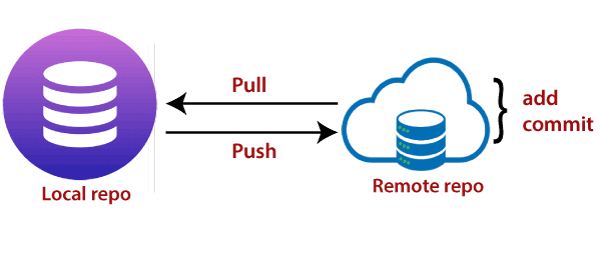
\includegraphics[width=0.6\textwidth,height=0.6\textheight,keepaspectratio]{figures/git-push.png}
\caption{Repositório local e remoto. Fonte \url{https://www.javatpoint.com/git-push}}
\label{fig-git-push}
\end{figure}

\end{frame}
\note{
Um repositório é o local para armazenar os dados 
relativos a um determinado projeto. É importante 
mantê-lo organizado e documentado. O repositório
poderá ser utilizado por diversos usuários no
desenvolvimento distribuído do projeto. 

Cada usuário do repositório terá a sua cópia local
dos dados.

O usuário deve
1. buscar novas atualizações no repositório remoto,
2. fazer suas modificações locais,
3. submetê-las para o repositório.

\begin{itemize}
\item Os repositórios podem ser públicos ou privados.
\item Repositórios públicos são acessíveis a qualquer um, 
basta para tanto ter a URL deste repositório.
\item O repositório pertence a um usuário ou à uma equipe.
\item Apenas o dono do repositório (ou o administrador, no 
caso de uma equipe) poderá apagar o repositório.
\item O código de um projeto pode consistir apenas dos dados
contidos em um único repositório, ou pode ser uma combinação
de múltiplos repositórios, mesmo que sejam de diferentes assinaturas 
(ou proprietários).
\end{itemize}
}

\begin{frame}
\frametitle{Git - hospedagem}
\begin{itemize}
\item GitHub
\item Bitbucket
\item SourceForge
\item Google Developers
\item GNU Savannah
\item GitLab
\item hospedagem local
\item outros
\end{itemize}

\vspace{2ex}
obs: OverLeaf utiliza git
\end{frame}



\begin{frame}
\frametitle{Esquema git}
\begin{figure}[h]
\centering
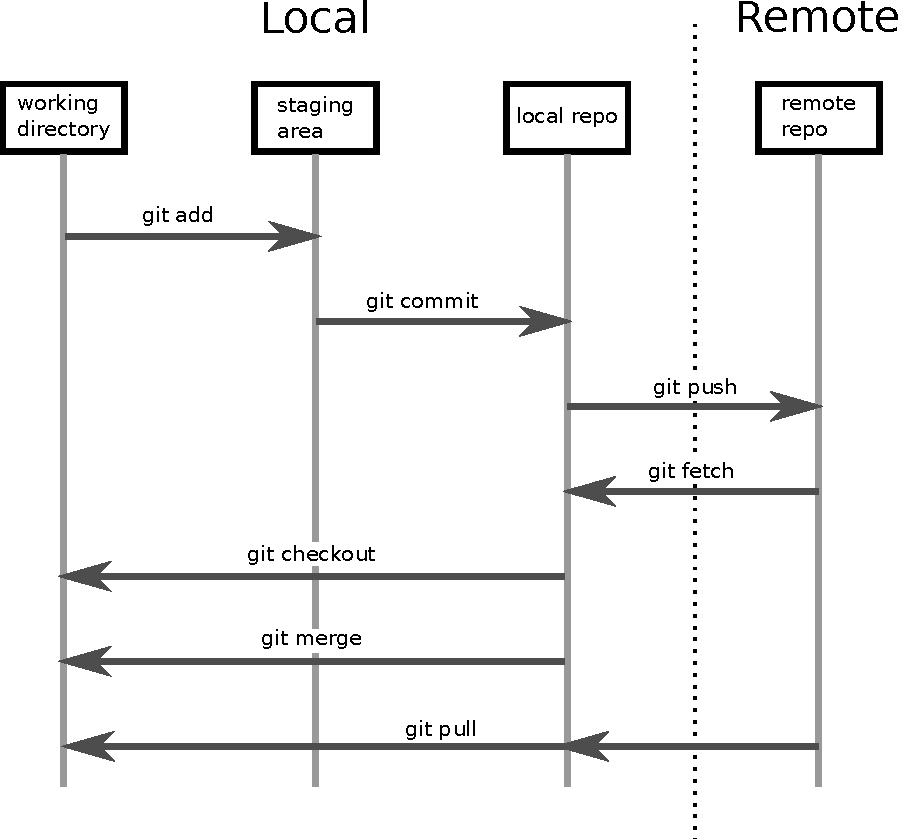
\includegraphics[width=0.8\textwidth,height=0.75\textheight,keepaspectratio]{figures/git-schema.pdf}
\caption{Esquema básico de utilização do git.}
\label{fig-git-schema}
\end{figure}
\end{frame}


\begin{frame}[fragile]
\frametitle{Criando um repositório local}
Inicialmente um repositório é vazio, mesmo que você
crie um repositório onde já existam arquivos.
Os arquivos deverão ser posteriormente adicionados 
ao repositório.

\begin{lstlisting}[language=bash, label=lst-git-repo, caption={Passos para criar um repositório local no Linux.}, postbreak=\mbox{$\hookrightarrow$\space}, basicstyle=\fontsize{8}{10}\selectfont\ttfamily]
# muda do diretorio corrente para o diretorio do repositorio
$ cd ~/myrepo
# inicializa o repositorio local
$ git init
# adiciona um arquivo e deixa-o pronto para o commit 
#               (perpetrar, alocar)
$ git add filename
# ou
# adiciona os arquivos no diretorio corrente
$ git add .
# realiza o commit dos aquivos preparados
$ git commit -m "mensagem de commit"
\end{lstlisting}
\end{frame}

\begin{frame}[fragile]
\frametitle{Repositório remoto}

\begin{lstlisting}[language=bash, label=lst-git-repo2, caption={Adicionando um repositório remoto.}, postbreak=\mbox{$\hookrightarrow$\space}, basicstyle=\fontsize{8}{10}\selectfont\ttfamily]
# adiciona o repositorio remoto
$ git remote add origin URL_do_repositiorio
# verificacao
$ git remote -v
# envia as modificacoes para o repositorio remoto
$ git push origin master
\end{lstlisting}
\end{frame}

\begin{frame}[fragile]
\frametitle{Clonando um repositório}
\begin{lstlisting}[language=bash, label=lst-git-repo2, caption={Clonando um repositório.}, postbreak=\mbox{$\hookrightarrow$\space}, basicstyle=\fontsize{8}{10}\selectfont\ttfamily]
$ git clone https://url_do_repositorio
# ou
$ git clone https://url_do_repositorio outro_nome
# caso queira dar outro nome ao diretorio
\end{lstlisting}

Será criado um diretório com o nome do repositório, inicializa-se o arquivo .git
e baixa todo o conteúdo do repositório.
\end{frame}


\begin{frame}[fragile]
\frametitle{Comandos básicos}

\begin{itemize}
\item \verb|git pull|
\item \verb|git status|
\item \verb|git add nome_do_arquivo|
\item \verb|git rm nome_do_arquivo|
\item \verb|git commit -m 'message'|
\item \verb|git push origin master|
\end{itemize}

\end{frame}



\begin{frame}
Sugestões de leitura: 
\vspace{2ex}

\fullcite{chacon_pro_2014}
\url{https://git-scm.com/book/en/v2}

\vspace{3ex}
\href{https://www.youtube.com/watch?v=xEKo29OWILE&list=PLHz_AreHm4dm7ZULPAmadvNhH6vk9oNZA}{Curso de Git e GitHub (Gustavo Guanabara)}

\end{frame}


